\chapter{Primitive Roots}\label{chapter:primitive-roots}

\section{Counting Elements of a Given Order Modulo a Prime}

\begin{figure}[t]
  \centering
  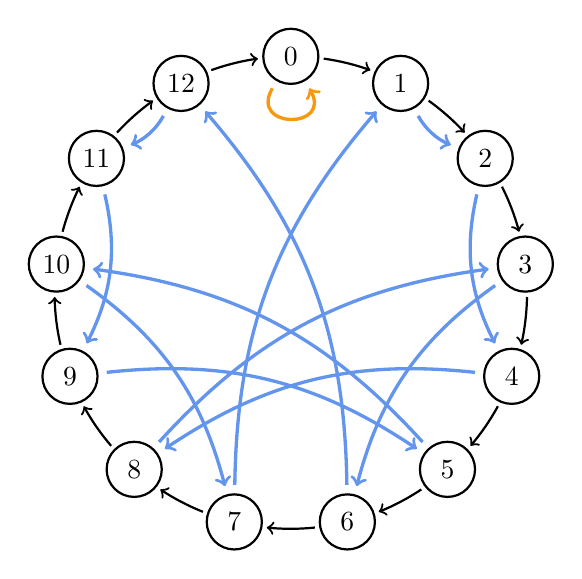
\begin{tikzpicture}[
    thick, every node/.style={circle, draw, minimum size=7mm, inner sep=1pt}]
    \def\n{13}
    \def\mult{2}
    \pgfmathtruncatemacro{\nminusone}{\n-1}
    \def\radius{3cm}
    
    \foreach \i in {0,...,\nminusone} {
      \pgfmathsetmacro{\value}{int(\i)}
      \node (N\i) at ({90-360/\n*(\i)}:\radius) {$\value$};
    }
    
    \foreach \i in {0,...,\nminusone} {
      \pgfmathsetmacro{\angle}{90-360/\n*(\i-1)}
      \draw[->] 
      ({\angle-8}:\radius)
      arc[start angle={\angle-8}, delta angle={-360/\n+16}, radius=\radius];
    }
    
    \draw[very thick,YellowOrange,->,shorten >= 3pt,shorten <= 3pt] (N0) to[out=240,in=300,looseness=5] (N0);
    
    \foreach \i in {1,...,\nminusone} {
      \pgfmathtruncatemacro{\j}{mod(\mult*\i,\n)}
      \pgfmathtruncatemacro{\d}{mod(\j-\i+\n,\n)}
      \pgfmathtruncatemacro{\useRight}{(\d <= \n/2 ? 1 : 0)}
      \ifnum\useRight=1
        \draw[very thick, CornflowerBlue, ->, shorten >= 3pt, shorten <= 3pt]
        (N\i) to[bend right=20] (N\j);
      \else
        \draw[very thick, CornflowerBlue, ->, shorten >= 3pt, shorten <= 3pt]
        (N\i) to[bend left=20] (N\j);
      \fi
    }
  \end{tikzpicture}  
  \caption[Doubling integers modulo $13$]{Doubling integers modulo $13$.}
  \label{figure:doubling-modulo-13}
\end{figure}

\crefnamed{theorem:eulers-theorem}{Euler's Theorem} tells us that
\begin{equation*}
  a^{\totient(n)}\equiv 1\pmod{n}
\end{equation*}
for every integer $a$ such that $\gcd(a,n)=1$. By the \crefnamed{theorem:order-theorem}{Order Theorem}, this implies that
\begin{equation*}
  \ord_n(a)\mid \totient(n).
\end{equation*}
Euler's theorem therefore gives an upper bound for the order of any element modulo $n$. For example, since $13$ is a prime number, we have $\totient(13)=12$, so all integers relatively prime to $13$ have an order dividing the number $12$. Computing the powers of $2$, for instance, we see that $\ord_{13}(2)=12$:
\begin{equation*}
    \newcolumntype{C}{>{\centering\arraybackslash$}m{1em}<{$}}
  \begin{tabular}{l*{12}{C}}
    $m$             & 0 & 1 & 2 & 3 & 4 & 5 & 6  & 7  & 8 & 9 & 10 & 11 \\ \midrule
    $2^m \pmod{13}$ & 1 & 2 & 4 & 8 & 3 & 6 & 12 & 11 & 9 & 5 & 10 & 7.
  \end{tabular}
\end{equation*}
The process of doubling integers modulo $13$ is illustrated in \cref{figure:doubling-modulo-13}. Using \cref{theorem:order-power}, we can use this table to compute the orders of all the nonzero integers modulo $13$. Recall that \cref{theorem:order-power} states that
\begin{equation*}
  \ord_n(a^m)=\frac{\ord_n(a)}{\gcd(m,\ord_n(a))}.
\end{equation*}
For example, since $3\equiv 2^4\pmod{13}$, it follows that the order of $3$ modulo $13$ is $3$. Similarly, since $5\equiv 2^9\pmod{13}$, it follows that
\begin{equation*}
  5^4 \equiv (2^9)^4 \equiv (2^{12})^3 \equiv 1 \pmod{13}.
\end{equation*}
Computing the orders of all the elements from $1$ to $12$ modulo $13$ this way, we obtain:
\begin{equation*}
  \newcolumntype{C}{>{\centering\arraybackslash$}m{1em}<{$}}
  \begin{tabular}{l*{12}{C}}
    $a$           & 1 & 2  & 3 & 4 & 5 & 6 & 7 & 8 & 9 & 10 & 11 & 12 \\ \midrule
    $\ord_{13}(a)$ & 1 & 12 & 3 & 6 & 4 & 12 & 12 & 4 & 3 & 6 & 12 & 2.
  \end{tabular}
\end{equation*}

While the orders of the integers modulo $13$ might at first glance appear to be somewhat unwieldy, \cref{theorem:order-power} is the key to some important patterns. For example, given an integer $a\pmod{p}$ with $\ord_p(a)=p-1$ such as $2\pmod{13}$, \cref{theorem:order-power} tells us that
\begin{equation*}
  \ord_p(a^m)=k \Leftrightarrow \frac{p-1}{\gcd(m,p-1)}=k
\end{equation*}
In particular, $\ord_p(a^m)=p-1$ if and only if $\gcd(m,p-1)=1$. Indeed, we see that there are four integers modulo $13$ of order $12$, corresponding to the powers of $2$ with exponents $1$, $5$, $7$, and $11$.

However, we can go further: There are two integers that have order $6$ modulo $13$, and indeed $\totient(6)=2$ as well. Similarly, we find that there are $\totient(1)$, $\totient(2)$, $\totient(3)$, and $\totient(4)$ integers of order $1$, $2$, $3$, and $4$, respectively. The following proposition tells us that modulo a prime $p$, the number of integers of order $k$ modulo $p$ is either $0$ or $\totient(k)$. This suggests that for any prime number $p$ and any $k\mid p-1$, it should be true that the number of elements of order $k$ is exactly $\totient(k)$. To make this observation precise, we first need a fundamental property of the totient function.

\begin{theorem}\label{theorem:dirichlet-convolution-phi}
  For every positive integer $n$, we have
  \begin{equation*}
    \sum_{d\mid n}\totient(d) = n,
  \end{equation*}
  where the sum ranges over the positive integers $d$ dividing $n$.
\end{theorem}

In terms of Dirichlet convolution, the identity in \cref{theorem:dirichlet-convolution-phi} can be stated as follows:
\begin{equation*}
  \totient\ast 1=\mathrm{id}.
\end{equation*}
We will give a combinatorial and an arithmetic proof.

\begin{proof}[Combinatorial proof]
  The sum suggests that there is a way of partitioning the set $\{1,\ldots,n\}$ into sets $A_d$ of size $\totient(d)$, and this is indeed how this theorem is proven. For each positive divisor $d$ of $n$, define the map
  \begin{equation*}
    f_d:{\textstyle \{1\leq x\leq  d \mid \gcd(x,d) = 1\}} \to \{1,\ldots,n\}
  \end{equation*}
  by $x\mapsto \frac{n}{d}x$, and define the set $A_d$ to be the image of $f_d$. Since $\frac{n}{d}$ is a positive integer, it follows that the map $f_d$ is injective, and therefore each set $A_d$ has exactly $\totient(d)$ elements. Now notice that
  \begin{equation*}
    y\in A_d \qquad\Leftrightarrow\qquad \gcd(y,n)=\frac{n}{d},
  \end{equation*}
  since if $x=y/\gcd(y,n)$, then $\gcd(x,d)=\gcd(y/\gcd(y,n),n/\gcd(y,n))=1$.
  Therefore, it follows that for every $1\leq y\leq n$ there is exactly one $d\mid n$ such that $y\in A_d$, so it follows that the sets $A_d$ partition the set $\{1,\ldots,n\}$. The sum of the numbers of elements of each $A_d$ is therefore $n$.
\end{proof}

\begin{proof}[Arithmetic proof]
  Recall from \cref{theorem:multiplicative-totient} that $\totient$ is a multiplicative function, which implies by \cref{theorem:multiplicative-functions} that the function
  \begin{equation*}
    n\mapsto \sum_{d\mid n}\totient(d)
  \end{equation*}
  is multiplicative. Since multiplicative functions are completely determined by their values on prime powers, it suffices to show that
  \begin{equation*}
    \sum_{d\mid p^m}\totient(d)=p^m.
  \end{equation*}
  The only divisors of $p^m$ are $p^k$ for $0\leq k\leq m$, and for any $k\geq 1$ we have $\totient(p^k)=p^k-p^{k-1}$. Thus, it follows that
  \begin{equation*}
    \sum_{d\mid p^m}\totient(d) = \sum_{k=0}^m\totient(p^k)= 1+\sum_{k=1}^m p^k-p^{k-1}=1+(p^m-1)=p^m.\qedhere
  \end{equation*}
\end{proof}

\begin{theorem}\label{theorem:count-integers-of-order-mod-prime}
  Consider a prime number $p$. Then there are for every $k\mid p-1$ exactly $\totient(k)$ integers of order $k$ modulo $p$.
\end{theorem}

The proof of this theorem makes essential use of the fact that any polynomial congruence of the form
\begin{equation*}
  x^d\equiv 1\pmod{p}
\end{equation*}
has at most $d$ solutions. This was established in \cref{theorem:maximal-number-of-roots-pow-minus-id}. To emphasize this observation, we will prove \cref{theorem:count-integers-of-order-mod-prime} as a consequence of the following more general theorem.

\begin{theorem}\label{theorem:count-integers-of-order}
  Consider a number $n$ with the property that every polynomial congruence of the form
  \begin{equation*}
    x^d\equiv 1\pmod{n}
  \end{equation*}
  has at most $d$ solutions. Then there are for every $k\mid\totient(n)$ exactly $\totient(k)$ integers of order $k$ modulo $n$.
\end{theorem}

\begin{proof}
  In this proof, let us write $\psi(k)$ for the number of integers of order $k$ modulo $n$. We claim that
  \begin{equation*}
    \psi(k)=
    \begin{cases}
      \totient(k) & \text{if $k\mid \totient(n)$,} \\
      0 & \text{otherwise.}
    \end{cases}
  \end{equation*}
  The fact that if $k\nmid \totient(n)$ then $\psi(k)=0$ follows immediately from the \crefnamed{theorem:order-theorem}{Order Theorem} and \crefnamed{theorem:fermats-little-theorem}{Fermat's Little Theorem}. Thus, it remains to show that $\psi(k)=\totient(k)$ for any $k\mid \totient(n)$.

  Consider an integer $a$ of order $k$ modulo $n$. By definition, every integer of order $k$ modulo $n$ is a solution to the polynomial congruence
  \begin{equation*}
    x^k\equiv 1 \pmod{n}.
  \end{equation*}
  This polynomial congruence has at most $k$ solutions. Given that the integer $a$ has order $k$ modulo $n$, we see that the set of solutions can be described exactly as the following set of numbers:
  \begin{equation*}
    1,~a,~\ldots,~a^{k-1}.
  \end{equation*}
  Thus, we see that every solution is congruent to a power of $a$. In particular, it follows that every integer of order $k$ modulo $n$ is itself a power of $a$. Recall from \cref{theorem:order-power} that an integer of the form $a^m$ has order $k$ if and only if $\gcd(m,k)=1$. Thus we conclude that, given an element of order $k$, there are exactly $\totient(k)$ integers of order $k$. In other words, $\psi(k)$ is either $0$ or $\totient(k)$, and certainly we have that $\psi(k)\leq \totient(k)$.

  To finish the proof, observe that, since every element $1\leq x<n$ relatively prime to $n$ has an order modulo $n$, we have
  \begin{equation*}
    \totient(n) =\sum_{k\mid \totient(n)}\psi(k)\leq \sum_{k\mid \totient(n)}\totient(k)=\totient(n).
  \end{equation*}
  It follows that the inequality is in fact an equality, and since $\psi(k)\leq \totient(k)$ for every $k\mid\totient(n)$ it follows that $\psi(k)=\totient(k)$ for every $k\mid \totient(n)$.
\end{proof}

\section{Primitive Roots}

We saw in the previous section that there are exactly $\totient(k)$ integers of order $k$ modulo $p$, for every $k\mid p-1$. It follows that there are
\begin{equation*}
  \totient(p-1)
\end{equation*}
integers of order $p-1$. Since $\totient(p-1)>0$, it follows that for every prime number $p$, there is an integer $g$ such that the integers
\begin{equation*}
  1,g,g^2,\ldots,g^{p-2}
\end{equation*}
form a reduced residue system modulo $p$. That is, there is an integer $g$ such that every integer $a$ relatively prime to $p$ is congruent to exactly one power $g^k$, where $0\leq k<p-1$. Such integers are called \emph{primitive roots}. In the previous section we saw that $2$ is a primitive root of the prime $13$. 

\begin{definition}
  A \emph{primitive root} modulo a natural number $n$ is an integer $g$ such that
  \begin{equation*}
    \ord_n(g)=\totient(n).
  \end{equation*}
\end{definition}

\begin{theorem}\label{theorem:primitive-roots}
  Consider a natural number $n$. The following are equivalent:
  \begin{enumerate}
  \item \label{itemi:primitive-roots}The number $n$ admits a primitive root modulo $n$.
  \item \label{itemii:primitive-roots}Any polynomial congruence of the form
    \begin{equation*}
      x^d\equiv 1\pmod{n}
    \end{equation*}
    has at most $d$ solutions.
%  \item \label{itemiii:primitive-roots}Unless $n\leq 2$, there is exactly one element of order $2$ modulo $n$.
  \end{enumerate}
  Furthermore, if the first condition holds then there are $\totient(\totient(n))$ primitive roots, and if the last condition holds and the polynomial congruence $x^d\equiv 1\pmod{n}$ has a solution, then it has exactly $\gcd(d,\totient(n))$ solutions.
\end{theorem}

\begin{proof}
  We have already proven that \ref{itemii:primitive-roots} implies \ref{itemi:primitive-roots} in \cref{theorem:count-integers-of-order}. To prove that \ref{itemi:primitive-roots} implies \ref{itemii:primitive-roots}, consider a primitive root $g$ modulo $n$, and consider the polynomial congruence
  \begin{equation*}
    x^d\equiv 1\pmod{n}.
  \end{equation*}
  An integer $a\equiv g^m\pmod{n}$ is a solution if and only if $g^{dm}\equiv 1\pmod{n}$. Since we assumed that $\ord_n(g)=\totient(n)$, it follows from the \crefnamed{theorem:order-theorem}{Order Theorem} that the congruence $g^{dm}\equiv 1\pmod{n}$ holds if and only if $\totient(n)\mid dm$. The number of $0\leq m<\totient(n)$ such that $\totient(n)\mid dm$ is exactly $\gcd(d,\totient(n))$, which is at most $d$. Therefore, it follows that there are at most $d$ solutions to the congruence $x^d\equiv 1\pmod{n}$.
\end{proof}

\begin{corollary}\label{corollary:primitive-roots-primes}
  The number of primitive roots of a prime number $p$ is $\totient(p-1)$. In particular, every prime $p$ admits a primitive root.
\end{corollary}

\begin{example}
  The number $9$ has the primitive root $2$. Indeed $\totient(9)=6$, and $2^3\equiv-1\pmod{9}$ so that $\ord_9(2)=6$. Thus, by the previous theorem it follows that the congruence $x^d\equiv 1\pmod{9}$ has at most $d$ solutions.

  Nevertheless, there are polynomials $f(x)$ of degree $2$ that are not of this form that have more than two solutions among the integers relatively prime to $9$. For example, the polynomial congruence
  \begin{equation*}
    x^2+x+7\equiv 0\pmod{9},
  \end{equation*}
  has the three solutions $x\equiv 1$, $4$, and $7\pmod{9}$.

  Some further composite numbers with primitive roots include $4$ and $6$: The number $3$ is a primitive root of $4$, and $5$ is a primitive root of $6$.

  The number $8$, on the other hand, does not have primitive roots because $\totient(8)=4$ while the odd integers $3$, $5$, and $7$ all have order $2$. In fact, it is possible to precisely classify all the natural numbers that have primitive roots. We will do so in \cref{theorem:moduli-with-primitive-roots}.
\end{example}

\section{The Discrete Logarithm}

It is useful to have access to primitive roots, if they exist, because if $g$ is a primitive root modulo $n$, then the integers
\begin{equation*}
  1,g,g^2,\ldots,g^{\totient(n)-1}
\end{equation*}
form a reduced residue system modulo $n$. This means that every number relatively prime to $n$ is congruent to exactly one of the integers $g^i$, for $0\leq i<\totient(n)$. Having a primitive root therefore gives a convenient way of representing all the elements of a reduced residue system.

\begin{definition}
  Suppose $g$ is a primitive root modulo $n$, and let $a$ be an integer relatively prime to $n$. Then we define the \emph{discrete logarithm} or \emph{index}
  \begin{equation*}
    \ind_g(a)
  \end{equation*}
  of $a$ base $g$ to be the unique integer $k$ modulo $\totient(n)$ such that $g^{k}=a$.
\end{definition}

\begin{theorem}
  Consider a natural number $n$ with a primitive root $g$.
  \begin{enumerate}
  \item For any two integers $a$ and $b$ relatively prime to $n$, we have
    \begin{equation*}
      a\equiv b\pmod{n}\qquad\Leftrightarrow\qquad\ind_g(a)\equiv\ind_g(b)\pmod{\totient(n)}.
    \end{equation*}
  \item Furthermore, we have
    \begin{align*}
      \ind_g(ab) & \equiv \ind_g(a)+\ind_g(b)\pmod{\totient(n)} \\
      \ind_g(a^m) & \equiv m\ind_g(a)\pmod{\totient(n)}.
    \end{align*}
  \end{enumerate}
\end{theorem}

\begin{example}
  Solving linear congruences becomes quite a straightforward task when a primitive root is known. For example, the congruence
  \begin{equation*}
    14x\equiv 6\pmod{26}
  \end{equation*}
  is solvable if and only if $7x\equiv 3\pmod{13}$ is. By the previous theorem, this linear congruence is equivalent to the linear congruence
  \begin{equation*}
    \ind_2(7)+\ind_2(x)\equiv\ind_2(3)\pmod{12}.
  \end{equation*}
  Since $\ind_2(7)=11$ and $\ind_2(3)=4$, we find that $\ind_2(x)\equiv 5\pmod{12}$. Thus, we conclude that
  \begin{equation*}
    x\equiv 6\pmod{13}
  \end{equation*}
  is a solution of the original linear congruence.
\end{example}

% \begin{theorem}
%   Consider a natural number $n$ that admits primitive roots, and let $a$ be relatively prime to $n$. Then the set
%   \begin{equation*}
%     I_a := \{0\leq k<\totient(n)\mid \text{there is a primitive root $g$ such that $g^k\equiv a\pmod{n}$}\}
%   \end{equation*}
%   has exactly $\totient(\ord_n(a))$ elements, the least of which is $\frac{\totient(n)}{\ord_n(a)}$.
% \end{theorem}

% \begin{theorem}
%   Suppose $n$ is a natural number that admits a primitive root and write $n=2^{\alpha}p^k$. Consider a polynomial $f(x)=a_dx^d+\cdots+a_0$ with integer coefficients so that the leading coefficient $a_d$ is relatively prime to $n$. Furthermore, assume that for every prime divisor $q\mid n$, the polynomials $f(x)$ and $f'(x)$ are relatively prime as polynomials. Then the number of roots of $f(x)$ modulo $n$ is at most $d$.
% \end{theorem}

\section{The Moduli with Primitive Roots}

We have established the existence of primitive roots modulo any prime. In this section, we will give a complete characterization of those moduli for which a primitive root exists.

\subsection{Primitive Roots Modulo Odd Prime Powers}
Our first target is to show that any odd prime power $p^k$ has a primitive root. Our approach to this problem is of an arithmetic nature, based on an analysis of the $p$-valuations of differences of powers.

For the following lemma, recall that $\nu_p(a-b)=m$ if and only if $a\equiv b\pmod{p^m}$ but $a\nequiv b\pmod{p^{m+1}}$. We also recall that for any prime $p$ and any $0<i<p$, the binomial coefficient $\binom{p}{i}$ is divisible by $p$. 

\begin{lemma}\label{lemma:lte-step}
  Consider an odd prime $p$, and two integers $a\equiv b\pmod{p}$ such that neither $a$ nor $b$ is divisible by $p$. Then
  \begin{equation*}
    \nu_p(a^p-b^p)=\nu_p(a-b)+1.
  \end{equation*}
\end{lemma}

\begin{proof}
  Write $s:=\nu_p(a-b)$, so that $s\geq 1$ by the assumption that $a\equiv b\pmod{p}$. Then we have $a\equiv b\pmod{p^s}$, so we can write $b=a+tp^s$, where $p\nmid t$. The value of $b^p$ can therefore be computed using the \crefnamed{theorem:binomial-theorem}{Binomial Theorem} by
  \begin{equation*}
    b^p=(a+tp^s)^p=\sum_{i=0}^p\binom{p}{i}a^i(tp^s)^{p-i} \equiv a^p+a^{p-1}tp^{s+1}\pmod{p^{s+2}}.
  \end{equation*}
  Since neither $a$ nor $t$ is divisible by $p$, it follows that $a^p\nequiv b^p\pmod{p^{s+2}}$. On the other hand, we see from the binomial expansion of $b^p$ that $a^p\equiv b^p\pmod{p^{s+1}}$. Therefore we conclude that
  \begin{equation*}
    \nu_p(a^p-b^p)=s+1.\qedhere
  \end{equation*}
\end{proof}

The previous lemma can be iterated to obtain a general lemma called the \emph{Lifting the Exponent Lemma}. This lemma was popularized by the Romanian mathematician Mihai Manea \cite{manea2006}.

\begin{lemma}[Lifting the Exponent]\label{lemma:lte}
  Consider an odd prime $p$, and let $x\equiv y\pmod{p}$, where neither $x$ nor $y$ is divisible by $p$. Then for any natural number $n\geq 1$, we have
  \begin{equation*}
    \nu_p(x^n-y^n)=\nu_p(x-y)+\nu_p(n).
  \end{equation*}
\end{lemma}

\begin{proof}
  Write $n=p^km$ with $p\nmid m$, so that $\nu_p(n)=k$, and write $s=\nu_p(x-y)$. Since we have assumed that $x\equiv y\pmod{p}$, we have $s\geq 1$. We will prove the claim by induction on $k$.

  In the base case, where $k=0$, the claim is simply that
  \begin{equation*}
    \nu_p(x^m-y^m)=s.
  \end{equation*}
  To see this, write $y=x+tp^s$, where $p\nmid t$. Then we have
  \begin{equation*}
    y^m=(x+tp^s)^m\equiv x^m+mx^{m-1}tp^s \pmod{p^{s+1}}.
  \end{equation*}
  Now observe that $m$, $x$, and $t$ are not divisible by $p$ by assumption, so it follows that $mx^{m-1}t$ is not divisible by $p$. This implies that $y^m\nequiv x^m\pmod{p^{s+1}}$. On the other hand, the congruence $x\equiv y\pmod{p^s}$ clearly implies that $x^m\equiv y^m\pmod{p^s}$, so we conclude that
  \begin{equation*}
    \nu_p(x^m-y^m)=s.
  \end{equation*}
  The inductive step is a direct consequence of \cref{lemma:lte-step}.
\end{proof}

Recall that for any integer $a$ not divisible by $p$, the integer $a^{p-1}-1$ is divisible by $p$ by \cref{theorem:fermats-little-theorem}. Therefore, its $p$-adic valuation $\alpha:=\nu_p(a^{p-1}-1)$ is at least $1$. In the following lemma we will establish that the order of $a$ modulo $p^k$ can be determined in terms of $\alpha$.

\begin{lemma}\label{lemma:order-modulo-prime-power-primitive-root}
  Consider an odd prime $p$ and a primitive root $g$ modulo $p$. Furthermore, let
  \begin{equation*}
    m:=\nu_p(g^{p-1}-1).
  \end{equation*}
  Then the order of $g$ modulo $p^k$ is $p^{\max(0,k-m)}(p-1)$. 
\end{lemma}

\begin{proof}
  First, we observe that $\ord_p(g)\mid \ord_{p^k}(g)$, so the order of $g$ modulo $p^k$ must be a multiple of $p-1$. Write $g^{p-1}=kp^{m}+1$, so that $p\nmid k$. By the \crefnamed{lemma:lte}{Lifting the Exponent Lemma} it follows that
  \begin{equation*}
    \nu_p(g^{p^t(p-1)}-1)=m+t.
  \end{equation*}
  Consequently, for any integer $s$ not divisible by $p$ we have
  \begin{equation*}
    g^{p^ts(p-1)}=(kp^{m+t}+1)^s\equiv 1+skp^{m+t}\pmod{p^{m+t+1}}.
  \end{equation*}
  This shows that $\nu_p(g^{p^ts(p-1)}-1)=m+t$ for such $s$. The first exponent $r$ such that $g^r\equiv 1\pmod{p^k}$ is therefore $r=p^{\max(0,k-m)}(p-1)$.
\end{proof}

\begin{theorem}\label{theorem:primitive-roots-odd-prime-powers}
  Any prime power $p^k$ with $k\geq 1$ admits a primitive root.
\end{theorem}

\begin{proof}
  By \cref{lemma:order-modulo-prime-power-primitive-root} it suffices to construct a primitive root $h$ modulo $p$ such that $\nu_p(h^{p-1}-1)=1$.

  Consider a primitive root $g$ modulo $p$. Write $g^{p-1}=kp+1$, and define $h_t:=g+tp$. Then we have
  \begin{equation*}
    h_t^{p-1}=(g+tp)^{p-1}\equiv g^{p-1}+(p-1)g^{p-2}tp\equiv 1+p(k-g^{p-2}t) \pmod{p^2}.
  \end{equation*}
  Thus we see that $h_t^{p-1}\equiv 1\pmod{p^2}$ if and only if
  \begin{equation*}
    k \equiv g^{p-2}t \pmod{p}.
  \end{equation*}
  This linear congruence has the unique solution $t\equiv kg\pmod{p}$. Thus we see that for any $t\nequiv kg\pmod{p}$, we have $h_t^{p-1}\nequiv 1\pmod{p^2}$ and hence
  \begin{equation*}
    \nu_p(h_t^{p-1}-1)=1.\qedhere
  \end{equation*}
\end{proof}

\subsection{The Complete Characterization of Moduli with Primitive Roots}

\begin{theorem}\label{theorem:moduli-with-primitive-roots}
  Consider a positive integer $n$. The following are equivalent:
  \begin{enumerate}
  \item \label{itemi:classification-primitive-roots}The number $n$ admits a primitive root.
  \item \label{itemii:classification-primitive-roots}Either $n=2$, or there is a unique element of order $2$ modulo $n$.
  \item \label{itemiii:classification-primitive-roots}We have
  \begin{equation*}
    n=2,~4,~p^k,~\text{or }~2p^k,
  \end{equation*}
  where $p$ is an odd prime.
  \end{enumerate}
\end{theorem}

\begin{proof}
  We saw in \cref{theorem:primitive-roots} that if $n$ admits a primitive root, then the congruence
  \begin{equation*}
    x^d\equiv 1\pmod{n}
  \end{equation*}
  had at most $d$ solutions, for any $d\geq 0$. In particular, there are at most two solutions to the congruence $x^2\equiv 1\pmod{n}$. One of them is the number $1$, which is of order $1$. The other is $-1$, which is of order $2$. Since any element of order $2$ is a solution to the congruence $x^2\equiv 1\pmod{n}$, we see that \ref{itemi:classification-primitive-roots} implies \ref{itemii:classification-primitive-roots}.

  Next, assume that there is a unique element of order $2$ modulo $n$. The case $n=4$ is swiftly dealt with, since $-1$ is the unique integer of order $2$ modulo $4$. If $n=2^k$ for some $k\geq 3$, then there are three integers of order $2$ modulo $2^k$:
  \begin{equation*}
    x=- 1\qquad\text{and}\qquad x=2^{k-1}\pm 1.
  \end{equation*}
  Thus we see that if $n=2^k$ for some $k\geq 3$, then $n$ does not satisfy the hypothesis in \ref{itemii:classification-primitive-roots}.

  Now suppose that $n=km$, where $\gcd(k,m)=1$ and $m$ is odd and strictly greater than $1$. By the \crefnamed{theorem:chinese-remainder-theorem}{Chinese Remainder Theorem}, it follows that any pair of solutions
  \begin{align*}
    x^2 & \equiv 1\pmod{k}, \\
    y^2 & \equiv 1\pmod{m},
  \end{align*}
  determines a unique solution to the congruence $z^2\equiv 1\pmod{km}$. It follows that one of them can have only one nontrivial solution. Since we assumed that $m>1$ is odd, and thus has two distinct solutions, it follows that there is only one solution to the congruence $x^2\equiv 1\pmod{k}$. Observe that there is only one such solution if and only if $k=1$ or $k=2$. Furthermore, the previous observation implies that $m$ cannot have distinct prime factors, so we conclude that $m$ must be of the form $m=p^k$ for some odd prime $p$. Thus we have proven that \ref{itemii:classification-primitive-roots} implies \ref{itemiii:classification-primitive-roots}.

  Finally, we have to show that any number of the form $n=2,4,p^k$, or $2p^k$, where $p$ is an odd prime, admits a primitive root. The number $1$ is a primitive root modulo $2$, and the number $-1$ is a primitive root modulo $4$. The fact that any odd prime power $p^k$ admits primitive roots was established in \cref{theorem:primitive-roots-odd-prime-powers}. To finish the proof that \ref{itemiii:classification-primitive-roots} implies \ref{itemi:classification-primitive-roots}, it therefore remains to show that each number of the form $n=2p^k$, where $p$ is an odd prime, has a primitive root. To see this, observe that the integers relatively prime to $2p^k$ are exactly the odd integers $1\leq x<2p^k$ relatively prime to $p^k$. Among those odd integers is a primitive root $g$ modulo $p^k$. Its order modulo $2p^k$ is
  \begin{equation*}
    \ord_{2p^k}(g)=\ord_{p^k}(g)=p^{k-1}(p-1)=\phi(2p^k),
  \end{equation*}
  so we see that $g$ is also a primitive root of $2p^k$.
\end{proof}

\section{A Criterion for Congruences of Degree \texorpdfstring{$n$}{n}}

While we are primarily interested in the quadratic congruence
\begin{equation*}
  x^2\equiv a\pmod{p}
\end{equation*}
in this introductory course on elementary number theory, the techniques that we have developed so far perfectly allow us to cover the $n$th degree congruence
\begin{equation*}
  x^n\equiv a\pmod{p}.
\end{equation*}
The following theorem is a significant generalization of \crefnamed{theorem:eulers-criterion}{Euler's Criterion}.

\begin{theorem}
  Consider an integer $a$ and a prime $p$ so that $p\nmid a$. The following are equivalent:
  \begin{enumerate}
  \item The congruence
    \begin{equation*}
      x^n\equiv a\pmod{p}
    \end{equation*}
    has a solution.
  \item The congruence
    \begin{equation*}
      \frac{p-1}{\ord_p(a)}\equiv 0\pmod{\gcd(n,p-1)}
    \end{equation*}
    holds.
  \item The congruence
    \begin{equation*}
      a^{\frac{p-1}{\gcd(n,p-1)}}\equiv 1\pmod{p}
    \end{equation*}
    holds.
  \end{enumerate}
  If the first condition holds, then the congruence $x^n\equiv a$ has exactly $d:=\gcd(n,p-1)$ solutions.
\end{theorem}

\begin{proof}[Proof by primitive roots]
  Let $m:=(p-1)/\ord_p(a)$, and consider a primitive root $g$ modulo $p$ such that
  \begin{equation*}
    g^{m}\equiv a\pmod{p}.
  \end{equation*}
  Then the congruence
  \begin{equation*}
    x^n\equiv a\pmod{p}
  \end{equation*}
  is solvable if there exists an integer $t$ such that
  \begin{equation*}
    g^{tn}\equiv g^m\pmod{p}.
  \end{equation*}
  In other words, the first congruence is solvable if and only if the congruence
  \begin{equation*}
    tn \equiv m\pmod{p-1}
  \end{equation*}
  is solvable. It follows from \cref{theorem:linear-congruence-one-variable} that this congruence is solvable if and only if $d:=\gcd(n,p-1)\mid m$, and in this case there are exactly $d$ solutions. Thus we have shown that {\it 1.}~is equivalent to {\it 2.}

  To show that {\it 3.}~is equivalent to {\it 2.}, consider the condition that
  \begin{equation*}
    a^{\frac{p-1}{\gcd(n,p-1)}}\equiv 1\pmod{p}.
  \end{equation*}
  This holds if and only if $\frac{m(p-1)}{\gcd(n,p-1)}$ is an integer multiple of $p-1$, which is equivalent to the condition that $\gcd(n,p-1)\mid m$.
\end{proof}

\begin{proof}[Proof by Lagrange's Theorem]
  For both directions of the proof, we will write $d:=\gcd(n,p-1)$, so that there are integers $k$ and $l$ such that $kd=p-1$ and $ld=n$. It follows that $k$ and $l$ are relatively prime, so that there are integers $u$ and $v$ such that
  \begin{equation*}
    ku+lv=1.
  \end{equation*}
  
  To prove the forward implication, assume that $x$ is an integer such that $x^n\equiv a\pmod{p}$. Then we have by \crefnamed{theorem:fermats-little-theorem}{Fermat's Little Theorem}
  \begin{equation*}
    a^k\equiv x^{kn}=x^{kld}=(x^{p-1})^l\equiv 1^l = 1\pmod{p}.
  \end{equation*}
  Since $k=(p-1)/\gcd(n,p-1)$, we have proven the forward implication.

  For the converse, assume that $a^k\equiv 1\pmod{p}$. Now we can use the formula for the difference of $k$th powers to write
  \begin{equation*}
    x^{p-1}-1=x^{kd}-1\equiv x^{kd}-a^k= (x^{d}-a)\sum_{i=0}^{k-1} x^{di}a^{k-1-i}.
  \end{equation*}
  Since the polynomial $x^{p-1}-1$ has exactly $p-1$ roots modulo $p$, it follows that the number of roots of each factor on the right-hand side is equal to its degree. In other words, the polynomial
  \begin{equation*}
    x^{d}-a
  \end{equation*}
  has $d$ roots. Given a root $x^d\equiv a\pmod{p}$, we define $y:=x^v$ where $ku+lv=1$. Then we have
  \begin{equation*}
    y^n=x^{vld}\equiv a^{lv} \equiv a^{1-ku} \equiv a(a^k)^{-u}\equiv a1^{-u}\equiv a\pmod{p}.\qedhere
  \end{equation*}
\end{proof}

\begin{corollary}
  Consider an integer $a$ such that $\ord_p(a)\mid n$. Then the congruence
  \begin{equation*}
    x^n\equiv a\pmod{p}
  \end{equation*}
  is solvable if and only if
  \begin{equation*}
    p\equiv 1\pmod{\ord_p(a)\cdot \gcd(n,p-1)}.
  \end{equation*}
\end{corollary}

\begin{corollary}
  Consider a prime $p$ and a natural number $n$ relatively prime to $p-1$. Then every $n$th degree congruence
  \begin{equation*}
    x^n\equiv a\pmod{p}
  \end{equation*}
  has a unique solution. In other words, the map $x\mapsto x^n$ is a bijection on $\mathbb{Z}/p\mathbb{Z}$.
\end{corollary}

In the following corollary, we show that the congruence $x^n\equiv -1\pmod{p}$ is solvable if and only if the $2$-adic valuation of $n$ is strictly smaller than the $2$-adic valuation of $p-1$. In other words, for any number $n=2^km$ with $m$ odd, the congruence
\begin{equation*}
  x^{n}\equiv -1\mod{p}
\end{equation*}
is solvable if and only if $p\equiv 1\pmod{2^{k+1}}$. 

\begin{corollary}
  The congruence
  \begin{equation*}
    x^n\equiv -1\pmod{p}
  \end{equation*}
  is solvable if and only if $\nu_2(n)<\nu_2(p-1)$. 
\end{corollary}

\begin{proof}
  Since the congruence $x^n\equiv -1\pmod{p}$ is solvable if and only if
  \begin{equation*}
    (-1)^{\frac{p-1}{\gcd(n,p-1)}}\equiv 1\pmod{p},
  \end{equation*}
  it suffices to show that the exponent $\frac{p-1}{\gcd(n,p-1)}$ is an even integer if and only if $\nu_2(n)<\nu_2(p-1)$. Indeed, this exponent is even if and only if $\min(\nu_2(n),\nu_2(p-1))=\nu_2(\gcd(n,p-1))<\nu_2(p-1)$. This strict inequality holds if and only if $\nu_2(n)<\nu_2(p-1)$.
\end{proof}

\exercises

\begin{starter}
  \exercise
  \begin{subexenum}
  \item Find the least primitive root $g$ modulo $23$, and give a table of the congruence classes of its powers.
  \item Find all primitive roots modulo $23$.
  \item For each $k\mid\totient(23)$, find all elements of order $k$ modulo $23$.
  \item For each integer $1,\ldots,22$, find its index base $g$ modulo $23$.
  \item Solve the linear congruence
    \begin{equation*}
      8x\equiv 9\pmod{23}
    \end{equation*}
    using indices.
  \end{subexenum}
  \exercise
  \begin{subexenum}
  \item Show that the number of solutions to the congruence
    \begin{equation*}
      x^n\equiv a\pmod{p}
    \end{equation*}
    is either $\gcd(n,p-1)$ or $0$.
  \item Find, as Gauss did in article 60 of \emph{Disquisitiones Arithmeticae} \cite{gauss1986}, all the solutions to the congruence
    \begin{equation*}
      x^{15}\equiv 11\pmod{19}.
    \end{equation*}
  \end{subexenum}
\end{starter}

\begin{routine}
  \exercise In article 55 of \emph{Disquisitiones Arithmeticae} \cite{gauss1986}, Gauss gives a second, more explicit construction of primitive roots. In this exercise we will follow this method.

  Consider a prime $p$ and suppose that the prime factorization of $p-1$ is
  \begin{equation*}
    p-1=q_1^{\alpha_1}\cdots q_n^{\alpha_n}.
  \end{equation*}
  \begin{subexenum}
  \item By \crefnamed{theorem:lagranges-theorem}{Lagrange's Theorem} it follows that for each prime $q_i$, the congruence
    \begin{equation*}
      x^{\frac{p-1}{q_i}}\equiv 1\pmod{p}
    \end{equation*}
    has strictly fewer than $p-1$ solutions, so there must exist a residue $x$ which is not a solution. Using such $x$, construct an element $a_i$ such that
    \begin{equation*}
      \ord_p(a_i)=q_i^{\alpha_i}.
    \end{equation*}
  \item Show that
    \begin{equation*}
      \ord_p(a_1\cdots a_n)=p-1
    \end{equation*}
    and conclude that the product $a_1\cdots a_n$ is a primitive root.
    \item Use this method to find a primitive root modulo $67$.
  \end{subexenum}
  \exercise Consider a prime $p\neq 3$. Prove that the product of all primitive roots modulo $p$ is congruent to $1$ modulo $p$.
  \exercise
  \begin{subexenum}
  \item Consider a prime number $p$. Show that the following are equivalent:
    \begin{enumerate}
    \item There is a solution to the congruence
      \begin{equation*}
        x^n\equiv a\pmod{p}
      \end{equation*}
      of the form $x=a^k$.
    \item The exponent $n$ is relatively prime to $\ord_p(a)$.
    \end{enumerate}
  \item Find a solution to the congruence
    \begin{equation*}
      x^3\equiv 5\pmod{13}
    \end{equation*}
    of the form $x=5^k$.
  \end{subexenum}
  \exercise Consider a prime $p$ with a primitive root $g$, and let $d\mid p-1$. Prove the congruence
  \begin{equation*}
    \sum_{\substack{0\leq m < p-1 \\ m\equiv 0\pmod{d}}}g^m\equiv \left\lfloor\frac{d}{p-1}\right\rfloor\pmod{p}.
  \end{equation*}
\end{routine}

\begin{challenge}
  \exercise \label{exercise:primitive-root-with-universal-exponent}For any prime $p$ and any integer $a$ not divisible by $p$, show that the number of primitive roots $g$ modulo $p$ such that
  \begin{equation*}
    g^{\frac{p-1}{\ord_p(a)}}\equiv a\pmod{p}.
  \end{equation*}
  is $\totient(p-1)/\totient(\ord_p(a))$. Conclude that such a primitive root always exists.
  \exercise Consider a prime $p>2$ and an odd number $m$. Show that the congruence $x^{2^nm}\equiv -1\pmod{p}$ is solvable if and only if $p\equiv 1\pmod{2^{n+1}}$.
  \exercise Consider a prime $p$ of the form $n^2+1$. Show that
  \begin{equation*}
    x^n\equiv a\pmod{p}\text{ is solvable}\qquad\Leftrightarrow\qquad a^n\equiv 1\pmod{p}.
  \end{equation*}
  \exercise \cite[art. 81]{gauss1986}~Consider a prime $p$. Prove that the sum of all primitive roots satisfies the following property:
  \begin{equation*}
    \sum_{g~\text{primitive root}\pmod{p}}g \equiv \mu(p-1)\pmod{p}.
  \end{equation*}
  \exercise \cite[art.~78]{gauss1986}~For any positive integer $n$, show that
  \begin{equation*}
    \prod_{\substack{0<x<n\\ \gcd(x,n)=1}} x \equiv
    \begin{cases}
      -1\pmod{n} & \text{if there is a primitive root modulo $n$,}\\
      1\pmod{n} & \text{otherwise.}
    \end{cases}
  \end{equation*}
  Hint: Use the \crefnamed{theorem:chinese-remainder-theorem}{Chinese Remainder Theorem} to show that the number of integers $0\leq x<n$ such that $x^2\equiv 1\pmod{n}$ is a power of $2$.
\end{challenge}

%%% Local Variables:
%%% mode: latex
%%% TeX-master: "elementary-number-theory"
%%% TeX-engine: luatex
%%% End:
